\section{Experiments}
\label{sec:experiments}

We apply MH-DIF to the METABENCH dataset~\citep{kipnis2024metabench}, which provides sparse response matrices for 5,227 models evaluated on 12,508 MMLU items~\citep{hendrycks2021mmlu}. All temporal analyses define reference and focal cohorts by model release date (2023 vs.\ 2024). We validate detection power through simulation, characterize temporal instability across multiple cohort designs, evaluate the relationship between DIF flags and existing contamination labels, and assess downstream consequences for benchmark rankings. Replication on GSM8K with cross-benchmark contamination validation appears in \Cref{sec:gsm8k}.

\subsection{Validation: DIF Detection Power}
\label{sec:validation}

To confirm that MH-DIF detects differential item functioning at the sample sizes available in METABENCH, we conduct a power analysis using empirical MMLU IRT parameters. We simulate item response matrices where a controlled subset of items has injected DIF of varying magnitude ($|\Delta_{\mathrm{MH}}| \geq 1.4$) and evaluate ETS~C classification across sample sizes $N \in \{40, 80, 160, 320\}$ per cohort. At $N \geq 80$, ETS~C achieves true positive rates of 0.68--0.80 with false positive rates of 0.036--0.042 and AUC of 0.93--0.94. The temporal cohort sizes in our analysis ($N_{\mathrm{ref}} = 1{,}080$, $N_{\mathrm{focal}} = 807$) far exceed this threshold, and statistical power is not a limiting factor for the results reported below. Full simulation results with confidence intervals appear in Appendix~Table~A1.

\subsection{Temporal Comparability: 31\% Item Instability}
\label{sec:temporal}

The central finding of this paper is that a substantial fraction of MMLU items behave differently across model generations. Comparing models released in 2023 ($N = 1{,}080$) against models released in 2024 ($N = 807$), 31.3\% of items receive ETS~C classification ($|\Delta_{\mathrm{MH}}| \geq 1.5$). Applying Benjamini-Hochberg FDR correction at $q = 0.05$ reduces this from 31.32\% to 31.30\%, removing only 3 items. The minimal impact of FDR correction reflects the fact that the ETS classification system imposes a dual threshold on both effect size and statistical significance, which already provides implicit multiple-testing protection. In absolute terms, nearly one in three MMLU items exhibits a large shift in its statistical relationship to overall model ability between the two cohort periods.

Three control conditions establish that this instability reflects genuine temporal change rather than methodological artifacts. A random split of the 2023 cohort into two equal halves produces only 0.18\% ETS~C items, confirming that sampling noise alone does not generate large-scale DIF. An ability-quintile comparison (lowest-scoring vs.\ highest-scoring models within the same temporal cohort) yields 2.9\% ETS~C items, indicating that ability differences alone are insufficient to produce the observed instability. A within-family comparison of Llama-2 ($N = 161$) and Llama-3 ($N = 308$) models produces 61.3\% ETS~C items. This elevated rate is consistent with the known sensitivity of MH-DIF to ability differences between groups~\citep{holland1988mh}: models from different generations within a single family exhibit large ability gaps that confound the DIF signal. The contrast between 2.9\% (ability-controlled) and 61.3\% (ability-confounded) brackets the temporal rate of 31.3\% and confirms that it captures a mixture of genuine item instability and residual ability differences.

The instability penetrates within every knowledge domain. Within-subject analysis yields an average of 38.1\% ETS~C items across all five MMLU subjects (range: 31--45\%), and the ecological correlation between subject-level accuracy improvement and subject-level C\% is $\rho = 0.307$ ($p = 0.02$). This ecological correlation could suggest that domains where models improved most also exhibit the most instability. Item-level logistic regression, however, reveals that domain accuracy improvement explains only 2.4 percentage points of the 31.3\% temporal C\% (pseudo $R^2 = 0.0007$; counterfactual C\% with domain improvement regressed out $= 29.0\%$). Of the observed instability, 92.4\% is unrelated to aggregate domain-level accuracy gains and instead reflects item-specific changes in how models interact with individual questions. After controlling for item difficulty and discrimination (pseudo $R^2 = 0.042$), the coefficient of domain improvement reverses sign (Simpson's paradox), further confirming that domain-level accuracy gains do not drive the observed instability.

Architecture heterogeneity is a non-issue for this analysis. The METABENCH MMLU population is 99.98\% decoder-only (5,226 of 5,227 models). Excluding the single encoder-decoder model yields C\% $= 31.32\%$ with Jaccard similarity of 1.0 between flagged item sets. Threshold sensitivity analysis confirms robustness across the full ETS range: C\% $= 48.9\%$ at $|\Delta_{\mathrm{MH}}| \geq 1.0$, $31.3\%$ at $\geq 1.5$ (the standard ETS~C threshold), $18.3\%$ at $\geq 2.0$, and $10.2\%$ at $\geq 2.5$. The qualitative conclusion holds at every threshold. \Cref{tab:temporal_landscape} summarizes the DIF landscape across all cohort comparisons.

\begin{table}[t]
\centering
\caption{DIF landscape across cohort definitions. ETS~C denotes the percentage of items with $|\Delta_{\mathrm{MH}}| \geq 1.5$. FPR is measured against Li et al.\ web-overlap labels on the ``clean'' (non-overlapping) subset. Enrichment is the ratio of observed to expected overlap between DIF flags and web-overlap labels.}
\label{tab:temporal_landscape}
\small
\begin{tabular}{lcccc}
\toprule
Cohort Definition & $N_{\mathrm{ref}}$ / $N_{\mathrm{focal}}$ & ETS~C (\%) & FPR (Li clean) & Enrichment \\
\midrule
Temporal (2023 vs.\ 2024) & 1,080 / 807 & 31.3 & 0.318 & 0.96 \\
Ability quintile (Q1--2 vs.\ Q4--5) & ${\sim}$2,600 / ${\sim}$2,600 & 2.9 & 0.027 & 1.19 \\
Within-family (Llama-2 vs.\ 3) & 161 / 308 & 61.3 & -- & -- \\
Random split (sanity) & 540 / 540 & 0.18 & -- & -- \\
Within-subject (avg, 5 subjects) & \textit{varies} & 38.1 & -- & -- \\
\bottomrule
\end{tabular}
\end{table}

\subsection{Ground Truth Mismatch}
\label{sec:groundtruth}

If DIF captures differential contamination, flagged items should overlap with independently identified contaminated items. We evaluate this hypothesis against the web-overlap labels of \citet{li2024contamination}, which classify MMLU items as ``contaminated'' based on verbatim matches in web training corpora. The enrichment ratio of DIF flags against these labels is 0.96 (\Cref{tab:temporal_landscape}), indistinguishable from chance. This null result does not indicate that DIF fails to detect contamination. Semi-synthetic injection experiments demonstrate a clear dose-response relationship: injecting controlled differential contamination at exploitation rate $p = 0.5$ produces $\Delta\mathrm{TPR} = {+}0.508$, and at $p = 1.0$, $\Delta\mathrm{TPR} = {+}0.674$ (\Cref{fig:dose_response}). The disconnect between DIF flags and web-overlap labels arises because the two methods answer fundamentally different questions.

Web-overlap labels measure \emph{global exposure}: whether an item exists in publicly accessible training data. DIF measures \emph{differential functioning}: whether an item's statistical relationship to overall ability changes across temporal cohorts. An item can be globally contaminated yet function identically across cohorts if all model generations have comparable access to the same training data. Conversely, an item can exhibit large DIF without any identifiable contamination source if changes in training methodology alter how models process certain question types. The Li et al.\ labels are therefore the wrong ground truth for evaluating a differential detection method: the near-chance enrichment is expected, not evidence of failure.

\begin{figure}[t]
\centering
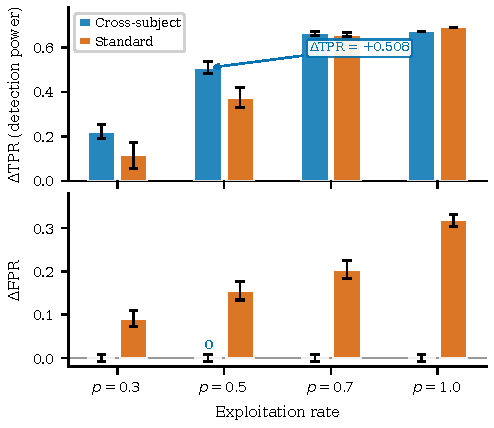
\includegraphics[width=\columnwidth]{fig_2_dose_response.pdf}
\caption{Semi-synthetic dose-response for DIF detection on MMLU. $\Delta\mathrm{TPR}$ increases monotonically with exploitation rate $p$, confirming that MH-DIF detects differential contamination when present. Baseline (no injection) produces $\Delta\mathrm{TPR} \approx 0$.}
\label{fig:dose_response}
\end{figure}

\subsection{Structural Analysis}
\label{sec:structural}

Three progressively refined approaches fail to reduce the temporal false positive rate below 31\%, revealing a structural property of the data rather than a methodological limitation. Matched-ability quintile analysis restricts comparisons to models of similar total score and yields enrichment ratios of 0.94--1.04, with temporal FPR unchanged at approximately 0.31. IRT $\theta$-conditioning with 20 ability strata achieves $r(\theta, \mathrm{total\ score}) = 0.9986$ and FPR $= 0.312$, confirming that the external total score already captures nearly all ability variance relevant to DIF computation. Within-subject DIF analysis, intended to isolate subject-specific effects, finds C\% $= 38.1\%$ across subjects, exceeding the 25\% threshold that would indicate viable bifactor structure. \Cref{tab:structural_comparison} summarizes these results. The temporal FPR reflects genuine item-level instability that persists regardless of how ability is measured or conditioned. Yen's Q3 diagnostic reveals mild local dependence within subjects (11.3\% of within-subject item pairs exceed $|Q3| > 0.20$, vs.\ 2.2\% cross-subject; $5{\times}$ ratio, $p = 2.3 \times 10^{-9}$), which contributes to elevated within-subject DIF rates but is not the primary driver: the cross-subject matching protocol addresses this bias, and temporal C\% persists under external matching (full Q3 distributions in Appendix~Figure~A2).

\begin{table}[t]
\centering
\caption{Structural approaches to reducing temporal DIF. None reduces baseline FPR below 31\%, indicating that the observed instability is not an artifact of ability matching. Subscript $\pm$ values denote standard deviations across 5 injection seeds (baseline row only).}
\label{tab:structural_comparison}
\small
\begin{tabular}{lcccc}
\toprule
Approach & Mechanism & Temporal FPR & TPR ($p{=}0.5$) & Outcome \\
\midrule
Baseline (external) & Cross-benchmark total score & $0.314_{\pm.009}$ & $0.834_{\pm.027}$ & Reference \\
Matched-ability & Within-quintile temporal DIF & ${\sim}$0.31 & -- & Enrich.\ 0.94--1.04 \\
$\theta$-conditioning & $\theta$ replaces total score & 0.312 & 0.876 & $r(\theta,\mathrm{total}) {=} 0.9986$ \\
Within-subject & Per-subject DIF & -- & -- & C\% $= 38.1\%$ ($>$25\%) \\
\bottomrule
\end{tabular}
\end{table}

\subsection{Semi-Synthetic Framework Validation}
\label{sec:semisynthetic}

The semi-synthetic injection framework enables controlled evaluation of DIF detection by flipping incorrect responses to correct for a designated ``contaminated'' subset of items in the focal cohort at a specified exploitation rate $p$. The critical methodological finding is that the choice of matching strategy determines whether the framework produces valid results. Cross-subject matching computes the matching variable from subjects \emph{other than} the one being tested, ensuring that the conditioning variable is unaffected by the injected contamination. Under this protocol, $\Delta\mathrm{FPR} = 0.000$ across all five MMLU subjects, and four of five subjects produce $\Delta\mathrm{TPR} > 0.3$ at $p = 0.5$ (\Cref{fig:within_subject}). Within-subject matching, by contrast, computes the matching variable from the same subject where contamination was injected, which inflates FPR by an average of ${+}0.186$ because the matching variable absorbs part of the injection signal and violates the conditional independence assumption of the MH procedure. We adopt cross-subject matching as the standard protocol for all subsequent analyses and recommend it as default for semi-synthetic DIF evaluation on multi-subject benchmarks.

\begin{figure}[t]
\centering

\includegraphics[width=\columnwidth]{fig_3_within_subject_matching.pdf}
\caption{Cross-subject vs.\ within-subject matching for semi-synthetic DIF detection. Cross-subject matching eliminates FPR inflation ($\Delta\mathrm{FPR} = 0.000$) while preserving detection power ($\Delta\mathrm{TPR} > 0.3$ for 4/5 subjects at $p = 0.5$). Within-subject matching inflates FPR by ${+}0.186$ on average.}
\label{fig:within_subject}
\end{figure}

\subsection{Downstream Impact}
\label{sec:downstream}

The practical relevance of 31\% item instability depends on whether unstable items affect model evaluation and benchmark rankings. We investigate this through a four-layer analysis that progresses from aggregate statistics to model-specific diagnostics.

\paragraph{Layer 1: Benchmark redundancy.} Spearman correlation between model rankings computed on all 12,508 items versus stable-only items (ETS~A/B) is $\rho \approx 0.997$. At the level of aggregate rankings, removing 31\% of items changes almost nothing. This redundancy is a consequence of the large item pool: 12,508 items provide sufficient statistical mass that removing nearly a third does not alter rank order.

\paragraph{Layer 2: Signal concentration with circularity check.} Despite aggregate redundancy, DIF-flagged items carry more discriminative signal than the average item. Removing DIF items degrades ranking discriminability more than removing an equal number of random items ($z = -8$ to $-49$ across 21 experimental conditions). A circularity ablation, however, places this in context: DIF-based removal is the \emph{least} disruptive among non-random removal strategies. Accuracy-gap removal produces $z = -156.5$, high-variance removal $z = -107.9$, and high-discrimination removal $z = -15.8$, compared to $z = -9.5$ for DIF removal. The Jaccard overlap between DIF-flagged and high-discrimination items is only 0.12. DIF items carry more signal than average, but DIF isolates differential behavior across cohorts specifically, not generally informative items.

\paragraph{Layer 3: Diagnostic lens.} Individual model families show distinctive DIF profiles that reveal which families disproportionately benefit from unstable items. Phi-3 and Llama-3 models gain ${+}700$ to ${+}850$ rank positions when evaluated on stable items only, suggesting inflated performance on items whose function changed between 2023 and 2024. Mistral-based model merges show the opposite pattern, losing $-400$ to $-587$ positions. A caveat applies: among the top 50 rank movers, most lack documented training details in METABENCH, limiting interpretation of what training choices drive these rank shifts.

\paragraph{Layer 4: Cross-benchmark signal.} The DIF instability pattern extends beyond MMLU. \Cref{sec:gsm8k} presents a full replication on GSM8K with independent contamination validation using the GSM1K held-out set~\citep{zhang2024gsm1k}. \Cref{fig:downstream} visualizes the relationship between full and DIF-filtered rankings.

\begin{figure}[t]
\centering

\includegraphics[width=\columnwidth]{fig_4_downstream_impact.pdf}
\caption{Downstream impact of DIF-based item filtering on model rankings. Despite $\rho \approx 0.997$ overall, individual model families show systematic rank shifts when evaluated on stable items only, with Phi-3 and Llama-3 gaining and Mistral merges losing rank positions.}
\label{fig:downstream}
\end{figure}

\subsection{Cross-Benchmark Validation: GSM8K}
\label{sec:gsm8k}

To test whether temporal DIF is specific to MMLU or reflects a broader phenomenon in LLM benchmarking, we replicate the full analysis pipeline on GSM8K (1,319 items $\times$ 6,702 models from METABENCH).

\paragraph{Temporal DIF.} Standard matching yields C\% $= 18.9\%$ for the temporal cohort comparison, with a random-split sanity check at 0.3\%. The lower instability rate compared to MMLU (31.3\%) is consistent with GSM8K's more homogeneous item structure: single-domain mathematical reasoning versus MMLU's 57 diverse subjects. The sanity check confirms that the signal is non-random.

\paragraph{Semi-synthetic validation.} Dose-response confirms detection power on this benchmark. Standard matching achieves $\Delta\mathrm{TPR} = {+}0.818$ at exploitation rate $p = 0.7$. External matching (using scores on ARC, HellaSwag, TruthfulQA, and Winogrande to match models) yields $\Delta\mathrm{TPR} = {+}0.514$ at $p = 0.5$, comparable to MMLU's ${+}0.508$ at the same exploitation rate, with $\Delta\mathrm{FPR}$ well-controlled. \Cref{tab:gsm8k_comparison} compares key metrics across both benchmarks.

\paragraph{GSM1K contamination gap.} The GSM1K dataset~\citep{zhang2024gsm1k} provides an independent measure of per-model contamination by comparing performance on the original GSM8K versus a held-out set of novel problems. For $N = 33$ models with both GSM1K scores and METABENCH evaluations, we correlate each model's contamination gap (GSM8K accuracy minus GSM1K accuracy) with the ranking advantage gained from DIF-flagged items. The observed correlation is $r = -0.478$ (95\% CI $= [-0.71, -0.16]$, $p = 0.005$; item-permutation $p = 0.014$), with partial $r = -0.385$ ($p = 0.027$) after controlling for overall accuracy. Our original hypothesis predicted a \emph{positive} correlation: models benefiting more from contamination should also benefit more from DIF items. The observed \emph{negative} correlation indicates the opposite. DIF-C items resist contamination-based performance gains, and models with larger contamination gaps benefit \emph{less} from these items. This result is suggestive at $N = 33$ and warrants replication with larger model populations, but it aligns with the broader interpretation that DIF captures item-level behavioral change distinct from simple memorization of training data. \Cref{fig:gsm1k} shows the correlation scatter.

\begin{figure}[t]
\centering

\includegraphics[width=\columnwidth]{fig_5_gsm1k_dif_correlation.pdf}
\caption{GSM1K contamination gap vs.\ DIF ranking advantage for $N = 33$ models. The negative correlation ($r = -0.478$, $p = 0.005$) indicates that models with larger contamination gaps benefit less from DIF-flagged items, contrary to the initial positive-correlation hypothesis.}
\label{fig:gsm1k}
\end{figure}

\begin{table}[t]
\centering
\caption{Cross-benchmark comparison of DIF analysis on MMLU and GSM8K. Both benchmarks exhibit temporal item instability with validated semi-synthetic detection power. Standard and external matching use different exploitation rates ($p$) because each benchmark's optimal operating point differs; external matching results are compared at $p = 0.5$ for both. Subscript $\pm$ values denote standard deviations across 5 random injection seeds.}
\label{tab:gsm8k_comparison}
\small
\begin{tabular}{lcc}
\toprule
Metric & MMLU & GSM8K \\
\midrule
Items & 12,508 & 1,319 \\
Models & 5,227 & 6,702 \\
Temporal C\% & 31.3\% & 18.9\% \\
Sanity C\% & 0.18\% & 0.3\% \\
$\Delta$TPR ($p{=}0.7$, standard) & -- & $+0.818_{\pm.006}$ \\
$\Delta$TPR ($p{=}0.5$, external) & $+0.508_{\pm.027}$ & $+0.514_{\pm.028}$ \\
\bottomrule
\end{tabular}
\end{table}
